% tikz_styles.tex
% TikZ Style Library for Mobile Anyons from Fusion Categories
% ============================================================
% This file provides a comprehensive collection of TikZ styles and macros
% for drawing fusion category diagrams, including:
%   - Fusion trees and morphism diagrams
%   - F-moves (associators) and pentagon equations
%   - R-moves (braiding) and hexagon equations
%   - Evaluation/coevaluation (cups and caps)
%   - Anyon chains and string diagrams

% ============================================================
% Required TikZ Libraries
% ============================================================
\usepackage{tikz}
\usetikzlibrary{
    positioning,           % Relative positioning
    shapes.geometric,      % Geometric shapes
    decorations.markings,  % Arrow decorations on paths
    decorations.pathmorphing, % Wavy/snake lines
    decorations.pathreplacing, % Braces
    arrows,                % Arrow tips
    arrows.meta,           % Modern arrow tips
    knots,                 % Knot crossings for braiding
    calc,                  % Coordinate calculations
    shapes,                % Additional shapes
    backgrounds,           % Background layers
    fit                    % Fitting nodes
}

% ============================================================
% Color Definitions
% ============================================================
% Professional color scheme: Complementary blue-orange with accents
% Based on color theory for scientific diagrams

% Primary pair (complementary)
\definecolor{AnyonBlue}{RGB}{41, 98, 155}       % Deep blue - primary
\definecolor{AnyonOrange}{RGB}{230, 126, 34}    % Warm orange - complement

% Secondary pair (split-complementary accents)
\definecolor{AnyonTeal}{RGB}{22, 160, 133}      % Teal - accent
\definecolor{AnyonCoral}{RGB}{192, 57, 43}      % Coral red - accent

% Neutral tones
\definecolor{AnyonSlate}{RGB}{52, 73, 94}       % Dark slate - for emphasis
\definecolor{AnyonSilver}{RGB}{149, 165, 166}   % Silver - subtle elements

% Background and UI colors
\definecolor{LightGray}{RGB}{236, 240, 241}     % Light background
\definecolor{MediumGray}{RGB}{189, 195, 199}    % Borders and lines

% Legacy aliases for backward compatibility
\definecolor{AnyonRed}{RGB}{192, 57, 43}        % Maps to AnyonCoral
\definecolor{AnyonGreen}{RGB}{22, 160, 133}     % Maps to AnyonTeal

% ============================================================
% Basic Arrow Styles for String Diagrams
% ============================================================
% Arrow at 60% along the path (standard direction)
\tikzset{->-/.style={
    decoration={markings, mark=at position .6 with {\arrow[>=stealth]{>}}},
    postaction={decorate}
}}

% Arrow at 52% (for certain diagram types)
\tikzset{-->--/.style={
    decoration={markings, mark=at position .52 with {\arrow[>=stealth]{>}}},
    postaction={decorate}
}}

% Reverse arrow at 60%
\tikzset{-<-/.style={
    decoration={markings, mark=at position .6 with {\arrow[>=stealth]{<}}},
    postaction={decorate}
}}

% Arrow at 50% (centered)
\tikzset{->>-/.style={
    decoration={markings, mark=at position .5 with {\arrow[>=stealth]{>}}},
    postaction={decorate}
}}

\tikzset{-<<-/.style={
    decoration={markings, mark=at position .5 with {\arrow[>=stealth]{<}}},
    postaction={decorate}
}}

% Arrow at different positions for longer strands
\tikzset{->>>-/.style={
    decoration={markings, mark=at position .5 with {\arrow[>=stealth]{>}}},
    postaction={decorate}
}}

\tikzset{-<<<-/.style={
    decoration={markings, mark=at position .4 with {\arrow[>=stealth]{<}}},
    postaction={decorate}
}}

% ============================================================
% Morphism Box Styles
% ============================================================
% Standard morphism box (gray rounded rectangle)
\tikzset{morphism box/.style={
    rectangle,
    draw,
    rounded corners,
    fill=LightGray,
    text centered,
    minimum height=0.7cm,
    minimum width=0.9cm,
    font=\small
}}

% Small morphism box
\tikzset{morphism box small/.style={
    morphism box,
    minimum height=0.5cm,
    minimum width=0.6cm,
    font=\scriptsize
}}

% Large morphism box (for composite morphisms)
\tikzset{morphism box large/.style={
    morphism box,
    minimum height=1cm,
    minimum width=1.2cm
}}

% ============================================================
% Fusion Vertex Styles
% ============================================================
% Filled vertex (standard trivalent vertex)
\tikzset{fusion vertex/.style={
    circle,
    fill=black,
    inner sep=1.5pt,
    outer sep=0pt
}}

% Empty vertex (for unfilled vertices)
\tikzset{fusion vertex empty/.style={
    circle,
    draw,
    fill=white,
    inner sep=1.5pt,
    outer sep=0pt
}}

% ============================================================
% Label Styles
% ============================================================
% Object labels (on strands)
\tikzset{object label/.style={
    font=\small,
    fill=white,
    inner sep=1pt
}}

% Vertex labels (multiplicity indices at vertices)
\tikzset{vertex label/.style={
    font=\tiny,
    fill=white,
    inner sep=0.5pt
}}

% Coefficient labels (for F-matrices, R-matrices)
\tikzset{coeff label/.style={
    font=\footnotesize,
    midway,
    fill=white,
    inner sep=1pt
}}

% ============================================================
% Commutative Diagram Arrow Style
% ============================================================
\tikzset{cd arrow/.style={
    ->,
    >=stealth,
    thick
}}

% Pentagon/Hexagon diagram arrow
\tikzset{
    pentagon arrow/.style={
        postaction={decorate},
        decoration={markings, mark=at position 1 with {\arrow[scale=1,thick]{>}}}
    }
}

% ============================================================
% MACROS FOR COMMON DIAGRAMS
% ============================================================

% ------------------------------------------------------------
% Trivalent Vertex (splitting): c -> a tensor b
% Usage: \trivalentvertex{a}{b}{c}
% ------------------------------------------------------------
\newcommand{\trivalentvertex}[3]{%
\begin{tikzpicture}[scale=0.7,baseline={(0,0.2)}]
    \draw (0,0) -- +(90:1) node[above] {\small $#3$};
    \draw (0,0) -- +(225:1) node[below] {\small $#1$};
    \draw (0,0) -- +(315:1) node[below] {\small $#2$};
\end{tikzpicture}%
}

% ------------------------------------------------------------
% Left-associative Fusion Tree: ((a,b)_e, c)_d
% Usage: \fuselefttree{a}{b}{e}{c}{d}
% ------------------------------------------------------------
\newcommand{\fuselefttree}[5]{%
\begin{tikzpicture}[scale=0.425,baseline={(0,0.4)}]
    \draw (0,0) node[below] {\small $#1$} -- (1.5,1.5) -- (3,0) node[below] {\small $#4$};
    \draw (0.75,0.75) -- (1.5,0) node[below] {\small $#2$};
    \draw (0.7,1.6) node {\small $#3$};
    \draw (1.5,1.5) -- (1.5,2.25) node[above] {\small $#5$};
\end{tikzpicture}%
}

% ------------------------------------------------------------
% Right-associative Fusion Tree: (a, (b,c)_e)_d
% Usage: \fuserighttree{a}{b}{e}{c}{d}
% ------------------------------------------------------------
\newcommand{\fuserighttree}[5]{%
\begin{tikzpicture}[scale=0.425,baseline={(0,0.4)}]
    \draw (0,0) node[below] {\small $#1$} -- (1.5,1.5) -- (3,0) node[below] {\small $#4$};
    \draw (2.25,0.75) -- (1.5,0) node[below] {\small $#2$};
    \draw (2.3,1.6) node {\small $#3$};
    \draw (1.5,1.5) -- (1.5,2.25) node[above] {\small $#5$};
\end{tikzpicture}%
}

% ------------------------------------------------------------
% F-move (Associator) Equation
% Displays: left tree = sum_f F * right tree
% Usage: \Fmoveequation{a}{b}{c}{d}{e}{f}
% ------------------------------------------------------------
\newcommand{\Fmoveequation}[6]{%
\begin{tikzpicture}[baseline=(current bounding box.center),scale=0.9]
    % Left tree: ((a b)_e c)_d
    \begin{scope}
        \draw (0,0.5) -- (0,1);
        \draw (0,1) -- (-0.5,1.5);
        \draw (-0.5,1.5) -- (-1,2);
        \draw (-0.5,1.5) -- (0,2);
        \draw (0,1) -- (0.5,1.5);
        \draw (0.5,1.5) -- (1,2);
        \node at (0,0.25) {\small $#4$};
        \node at (-1,2.25) {\small $#1$};
        \node at (0,2.25) {\small $#2$};
        \node at (1,2.25) {\small $#3$};
        \node at (-0.5,1.1) {\small $#5$};
    \end{scope}
    % Equals sign with proper spacing (anchor west for left-alignment)
    \node[anchor=west] at (1.4,1.25) {$=\displaystyle\sum_{#6} \left(F_{#4}^{#1#2#3}\right)_{#6#5}$};
    % Right tree: (a (b c)_f)_d - shifted further right
    \begin{scope}[xshift=6.2cm]
        \draw (0,0.5) -- (0,1);
        \draw (0,1) -- (-0.5,1.5);
        \draw (-0.5,1.5) -- (-1,2);
        \draw (0.5,1.5) -- (0,2);
        \draw (0,1) -- (0.5,1.5);
        \draw (0.5,1.5) -- (1,2);
        \node at (0,0.25) {\small $#4$};
        \node at (-1,2.25) {\small $#1$};
        \node at (0,2.25) {\small $#2$};
        \node at (1,2.25) {\small $#3$};
        \node at (0.5,1.1) {\small $#6$};
    \end{scope}
\end{tikzpicture}%
}

% ------------------------------------------------------------
% F-move with Multiplicity Indices
% For categories with N^c_{ab} > 1, vertices carry multiplicity labels
% Usage: \Fmovemult{a}{b}{c}{d}{e}{f}{mu}{nu}
% mu labels the (a,b)->e vertex, nu labels the (e,c)->d vertex on left
% On right: mu' labels (b,c)->f, nu' labels (a,f)->d
% ------------------------------------------------------------
\newcommand{\Fmovemult}[8]{%
\begin{tikzpicture}[baseline=(current bounding box.center),scale=0.9]
    % Left tree: ((a b)_e c)_d with multiplicities mu, nu
    \begin{scope}
        \draw (0,0.5) -- (0,1);
        \draw (0,1) -- (-0.5,1.5);
        \draw (-0.5,1.5) -- (-1,2);
        \draw (-0.5,1.5) -- (0,2);
        \draw (0,1) -- (0.5,1.5);
        \draw (0.5,1.5) -- (1,2);
        % Object labels
        \node at (0,0.25) {\small $#4$};
        \node at (-1,2.25) {\small $#1$};
        \node at (0,2.25) {\small $#2$};
        \node at (1,2.25) {\small $#3$};
        \node at (-0.75,1.1) {\small $#5$};
        % Multiplicity labels at vertices
        \node[fill=white,inner sep=1pt] at (-0.5,1.5) {\tiny $#7$};
        \node[fill=white,inner sep=1pt] at (0,1) {\tiny $#8$};
    \end{scope}
    % Equals sign with F-symbol including multiplicities
    \node[anchor=west] at (1.4,1.25) {$=\displaystyle\sum_{#6,#7',#8'} \left(F_{#4}^{#1#2#3}\right)_{#5#6}^{#7#8,#7'#8'}$};
    % Right tree: (a (b c)_f)_d with multiplicities mu', nu'
    \begin{scope}[xshift=7.5cm]
        \draw (0,0.5) -- (0,1);
        \draw (0,1) -- (-0.5,1.5);
        \draw (-0.5,1.5) -- (-1,2);
        \draw (0.5,1.5) -- (0,2);
        \draw (0,1) -- (0.5,1.5);
        \draw (0.5,1.5) -- (1,2);
        % Object labels
        \node at (0,0.25) {\small $#4$};
        \node at (-1,2.25) {\small $#1$};
        \node at (0,2.25) {\small $#2$};
        \node at (1,2.25) {\small $#3$};
        \node at (0.75,1.1) {\small $#6$};
        % Multiplicity labels at vertices (primed)
        \node[fill=white,inner sep=1pt] at (0.5,1.5) {\tiny $#7'$};
        \node[fill=white,inner sep=1pt] at (0,1) {\tiny $#8'$};
    \end{scope}
\end{tikzpicture}%
}

% ------------------------------------------------------------
% Simple F-move trees (without equation, for inline use)
% Usage: \Ftreeleft{a}{b}{c}{d}{e}{mu}{nu} and \Ftreeright{a}{b}{c}{d}{f}{mu}{nu}
% ------------------------------------------------------------
\newcommand{\Ftreeleft}[7]{%
\begin{tikzpicture}[baseline=(current bounding box.center),scale=0.7]
    \draw (0,0) -- (0,0.5);
    \draw (0,0.5) -- (-0.5,1);
    \draw (-0.5,1) -- (-1,1.5);
    \draw (-0.5,1) -- (0,1.5);
    \draw (0,0.5) -- (0.5,1);
    \draw (0.5,1) -- (1,1.5);
    \node at (0,-0.25) {\small $#4$};
    \node at (-1,1.75) {\small $#1$};
    \node at (0,1.75) {\small $#2$};
    \node at (1,1.75) {\small $#3$};
    \node at (-0.7,0.6) {\small $#5$};
    \node[fill=white,inner sep=1pt] at (-0.5,1) {\tiny $#6$};
    \node[fill=white,inner sep=1pt] at (0,0.5) {\tiny $#7$};
\end{tikzpicture}%
}

\newcommand{\Ftreeright}[7]{%
\begin{tikzpicture}[baseline=(current bounding box.center),scale=0.7]
    \draw (0,0) -- (0,0.5);
    \draw (0,0.5) -- (-0.5,1);
    \draw (-0.5,1) -- (-1,1.5);
    \draw (0.5,1) -- (0,1.5);
    \draw (0,0.5) -- (0.5,1);
    \draw (0.5,1) -- (1,1.5);
    \node at (0,-0.25) {\small $#4$};
    \node at (-1,1.75) {\small $#1$};
    \node at (0,1.75) {\small $#2$};
    \node at (1,1.75) {\small $#3$};
    \node at (0.7,0.6) {\small $#5$};
    \node[fill=white,inner sep=1pt] at (0.5,1) {\tiny $#6$};
    \node[fill=white,inner sep=1pt] at (0,0.5) {\tiny $#7$};
\end{tikzpicture}%
}

% ------------------------------------------------------------
% Evaluation (Cup): X* tensor X -> 1
% Usage: \evalcup{X}
% ------------------------------------------------------------
\newcommand{\evalcup}[1]{%
\begin{tikzpicture}[scale=0.85,baseline=(current bounding box.center)]
    \node at (-0.3,0) {$#1^*$};
    \node at (1.7,0) {$#1$};
    \draw (0,0) arc (180:0:0.7);
\end{tikzpicture}%
}

% ------------------------------------------------------------
% Coevaluation (Cap): 1 -> X tensor X*
% Usage: \coevalcap{X}
% ------------------------------------------------------------
\newcommand{\coevalcap}[1]{%
\begin{tikzpicture}[scale=0.85,baseline=(current bounding box.center)]
    \node at (-0.3,0) {$#1$};
    \node at (1.7,0) {$#1^*$};
    \draw (0,0) arc (-180:0:0.7);
\end{tikzpicture}%
}

% ------------------------------------------------------------
% Left Zigzag Identity (Snake equation)
% Usage: \leftzigzag{X}
% ------------------------------------------------------------
\newcommand{\leftzigzag}[1]{%
\begin{tikzpicture}[baseline=(current bounding box.center)]
    \draw (0,0) -- (0,1);
    \draw (0,1) arc (0:180:0.4);
    \draw (-0.8,1) arc (0:-180:0.4);
    \draw (-1.6,1) -- (-1.6,2);
    \node at (0.25,0) {$#1$};
    \node at (-1.85,2) {$#1$};
    \node at (-1.05,1) {$#1^*$};
\end{tikzpicture}%
}

% ------------------------------------------------------------
% Right Zigzag Identity (Snake equation)
% Usage: \rightzigzag{X}
% ------------------------------------------------------------
\newcommand{\rightzigzag}[1]{%
\begin{tikzpicture}[baseline=(current bounding box.center)]
    \draw (0,0) -- (0,1);
    \draw (0,1) arc (180:0:0.4);
    \draw (0.8,1) arc (-180:0:0.4);
    \draw (1.6,1) -- (1.6,2);
    \node at (-0.25,0) {$#1^*$};
    \node at (1.85,2) {$#1^*$};
    \node at (1.05,1) {$#1$};
\end{tikzpicture}%
}

% ------------------------------------------------------------
% Simple Braiding (Over-crossing): X crosses over Y
% Usage: \braidingover{X}{Y}
% ------------------------------------------------------------
\newcommand{\braidingover}[2]{%
\begin{tikzpicture}[scale=0.85,baseline=(current bounding box.center)]
    \node at (-0.75,0.35) {$#1$};
    \node at (-0.75,2.65) {$#2$};
    \node at (0.75,0.35) {$#2$};
    \node at (0.75,2.65) {$#1$};
    \draw (-0.4,0.2) -- (-0.4,0.5);
    \draw (-0.4,2.5) -- (-0.4,2.8);
    \draw (0.4,0.2) -- (0.4,0.5);
    \draw (0.4,2.5) -- (0.4,2.8);
    \begin{knot}[flip crossing/.list={8},consider self intersections=true,ignore endpoint intersections=false]
        \strand (-0.4,0.5)to[out=90,in=270](0.4,2.5);
        \strand (0.4,0.5)to[out=90,in=270](-0.4,2.5);
    \end{knot}
\end{tikzpicture}%
}

% ------------------------------------------------------------
% Inverse Braiding (Under-crossing): X crosses under Y
% Usage: \braidingunder{X}{Y}
% ------------------------------------------------------------
\newcommand{\braidingunder}[2]{%
\begin{tikzpicture}[scale=0.85,baseline=(current bounding box.center)]
    \node at (-0.75,0.35) {$#2$};
    \node at (-0.75,2.65) {$#1$};
    \node at (0.75,0.35) {$#1$};
    \node at (0.75,2.65) {$#2$};
    \draw (-0.4,0.2) -- (-0.4,0.5);
    \draw (-0.4,2.5) -- (-0.4,2.8);
    \draw (0.4,0.2) -- (0.4,0.5);
    \draw (0.4,2.5) -- (0.4,2.8);
    \begin{knot}[flip crossing/.list={8},consider self intersections=true,ignore endpoint intersections=false]
        \strand (0.4,0.5)to[out=90,in=270](-0.4,2.5);
        \strand (-0.4,0.5)to[out=90,in=270](0.4,2.5);
    \end{knot}
\end{tikzpicture}%
}

% ------------------------------------------------------------
% Compact Braiding for Hamiltonian terms (no labels, squatter)
% Usage: \braidcompact (over), \braidcompactinv (under)
% These fit nicely inside \left( \right) brackets
% ------------------------------------------------------------
\newcommand{\braidcompact}{%
\begin{tikzpicture}[scale=0.5,baseline={([yshift=-2pt]current bounding box.center)}]
    \begin{knot}[flip crossing/.list={1},consider self intersections=true,ignore endpoint intersections=false,clip width=3]
        \strand (0,0) to[out=90,in=270] (0.8,1.2);
        \strand (0.8,0) to[out=90,in=270] (0,1.2);
    \end{knot}
\end{tikzpicture}%
}

\newcommand{\braidcompactinv}{%
\begin{tikzpicture}[scale=0.5,baseline={([yshift=-2pt]current bounding box.center)}]
    \begin{knot}[consider self intersections=true,ignore endpoint intersections=false,clip width=3]
        \strand (0,0) to[out=90,in=270] (0.8,1.2);
        \strand (0.8,0) to[out=90,in=270] (0,1.2);
    \end{knot}
\end{tikzpicture}%
}

% ------------------------------------------------------------
% Labeled Compact Braiding (squatter, for Hamiltonian terms)
% Usage: \braidlabeled{X}{Y} (over), \braidlabeledinv{X}{Y} (under)
% ------------------------------------------------------------
\newcommand{\braidlabeled}[2]{%
\begin{tikzpicture}[scale=0.55,baseline={([yshift=-2pt]current bounding box.center)}]
    \node at (-0.3,-0.15) {\tiny $#1$};
    \node at (1.1,-0.15) {\tiny $#2$};
    \begin{knot}[flip crossing/.list={1},consider self intersections=true,ignore endpoint intersections=false,clip width=3]
        \strand (0,0) to[out=90,in=270] (0.8,1.2);
        \strand (0.8,0) to[out=90,in=270] (0,1.2);
    \end{knot}
\end{tikzpicture}%
}

\newcommand{\braidlabeledinv}[2]{%
\begin{tikzpicture}[scale=0.55,baseline={([yshift=-2pt]current bounding box.center)}]
    \node at (-0.3,-0.15) {\tiny $#2$};
    \node at (1.1,-0.15) {\tiny $#1$};
    \begin{knot}[consider self intersections=true,ignore endpoint intersections=false,clip width=3]
        \strand (0,0) to[out=90,in=270] (0.8,1.2);
        \strand (0.8,0) to[out=90,in=270] (0,1.2);
    \end{knot}
\end{tikzpicture}%
}

% ------------------------------------------------------------
% Twist (Ribbon element): curl on a single strand
% Usage: \twist{X}
% ------------------------------------------------------------
\newcommand{\twist}[1]{%
\begin{tikzpicture}[scale=1.1,baseline=(current bounding box.center)]
    \node at (1,0.7)[left] {$#1$};
    \begin{knot}[flip crossing/.list={4,5},consider self intersections=true,ignore endpoint intersections=false]
        \strand (1,0.5)--(1,1);
        \strand (1,1)to[out=90,in=180](1.25,1.75)to[out=0,in=90](1.45,1.5)to[out=270,in=0](1.25,1.25)to[out=180,in=270](1,2);
        \strand (1,2)--(1,2.5);
    \end{knot}
\end{tikzpicture}%
}

% ------------------------------------------------------------
% Bigon (Bubble): a,b fuse to c then split back
% Usage: \bigon{a}{b}{c}
% ------------------------------------------------------------
\newcommand{\bigon}[3]{%
\begin{tikzpicture}[baseline=(current bounding box.center)]
    \draw (0,0) -- (0,0.5);
    \draw (0,0.5) to[bend left=60] node[left] {$#1$} (0,1.5);
    \draw (0,0.5) to[bend right=60] node[right] {$#2$} (0,1.5);
    \draw (0,1.5) -- (0,2);
    \node at (0,-0.25) {$#3$};
    \node at (0,2.25) {$#3$};
\end{tikzpicture}%
}

% ------------------------------------------------------------
% Quantum Dimension Loop: closed loop labeled X
% Usage: \qdimloop{X}
% ------------------------------------------------------------
\newcommand{\qdimloop}[1]{%
\begin{tikzpicture}[baseline=(current bounding box.center)]
    \draw (0,0) circle (0.5cm);
    \node at (0.75,0) {$#1$};
\end{tikzpicture}%
}

% ------------------------------------------------------------
% Identity Strand: straight vertical line
% Usage: \identitystrand{X}
% ------------------------------------------------------------
\newcommand{\identitystrand}[1]{%
\begin{tikzpicture}[baseline=(current bounding box.center)]
    \draw (0,0) -- (0,2);
    \node at (-0.25,0) {$#1$};
    \node at (-0.25,2) {\phantom{$#1$}};
\end{tikzpicture}%
}

% ------------------------------------------------------------
% Anyon Chain Segment: N anyons with fusion labels
% Usage: Place manually or use as template
% ------------------------------------------------------------
\newcommand{\anyonchain}[1]{%
% Draws anyon chain with anyons living in INTERVALS (not at vertices)
% Vertical tick marks pass through the horizontal line to indicate lattice sites
% Anyons occupy the cells between ticks
\begin{tikzpicture}[scale=1.2,baseline=(current bounding box.center)]
    % Horizontal line (the chain)
    \draw (0,0) -- (3.2,0);
    \node at (3.5,0) {$\cdots$};
    % Vertical tick marks at lattice sites (pass through the line)
    \foreach \x in {0,1,2,3} {
        \draw (\x,-0.12) -- (\x,0.12);
    }
    % Anyon labels in intervals (centered between ticks)
    \node at (0.5,+0.3) {\small $#1_1$};
    \node at (1.5,+0.3) {\small $#1_2$};
    \node at (2.5,+0.3) {\small $#1_3$};
\end{tikzpicture}%
}

% Alternative: anyon chain with shaded intervals
\newcommand{\anyonchainshaded}[1]{%
\begin{tikzpicture}[scale=1.2,baseline=(current bounding box.center)]
    % Shaded intervals to show anyon locations
    \fill[AnyonBlue,opacity=0.15] (0,-0.15) rectangle (1,0.15);
    \fill[AnyonOrange,opacity=0.15] (1,-0.15) rectangle (2,0.15);
    \fill[AnyonBlue,opacity=0.15] (2,-0.15) rectangle (3,0.15);
    % Horizontal line
    \draw (0,0) -- (3.2,0);
    \node at (3.5,0) {$\cdots$};
    % Vertical tick marks at lattice sites
    \foreach \x in {0,1,2,3} {
        \draw (\x,-0.15) -- (\x,0.15);
    }
    % Anyon labels in intervals
    \node at (0.5,+0.35) {\small $#1_1$};
    \node at (1.5,+0.35) {\small $#1_2$};
    \node at (2.5,+0.35) {\small $#1_3$};
\end{tikzpicture}%
}

% ------------------------------------------------------------
% Splitting Tree: General N-particle splitting
% Usage: Manual construction using standard TikZ
% Template provided as example
% ------------------------------------------------------------
% Example usage for 4-particle splitting tree:
% \begin{tikzpicture}[scale=0.8]
%     \draw (0,0) -- (0,0.5);
%     \draw (0,0.5) -- (-0.5,1);
%     \draw (0,0.5) -- (0.5,1);
%     \draw (-0.5,1) -- (-1,1.5);
%     \draw (-0.5,1) -- (0,1.5);
%     \draw (0.5,1) -- (0.5,1.5);
%     \node at (0,-0.25) {$u$};
%     \node at (-1,1.75) {$a$};
%     \node at (0,1.75) {$b$};
%     \node at (0.5,1.75) {$c$};
%     \node at (-0.55,0.7) {\small $e$};
% \end{tikzpicture}

% ============================================================
% Circled Numbers (for numbered items in diagrams)
% ============================================================
\newcommand{\circlednum}[1]{%
\begin{tikzpicture}[baseline={([yshift=-3pt]current bounding box.center)}]
    \node[circle,scale=0.6,draw] at (0,0) {$#1$};
\end{tikzpicture}%
}

\newcommand{\circlednumcolor}[2]{%
\begin{tikzpicture}[baseline={([yshift=-3pt]current bounding box.center)}]
    \node[circle,scale=0.6,draw=#1] at (0,0) {$#2$};
\end{tikzpicture}%
}

% ============================================================
% Diamond Labels (for F-symbol indices)
% ============================================================
\newcommand{\Fdiamond}[1]{%
\begin{tikzpicture}[baseline={([yshift=-3pt]current bounding box.center)},scale=1]
    \node[diamond,scale=0.35,draw,black] at (0,0) {\huge $#1$};
\end{tikzpicture}%
}

% ============================================================
% Temperley-Lieb Patterns
% ============================================================
% Two parallel arcs (TL identity)
\newcommand{\TLidentity}{%
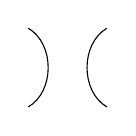
\begin{tikzpicture}[baseline={([yshift=-3pt]current bounding box.center)}]
    \draw (0,0) to [bend right=60] (0,1);
    \draw (1,0) to [bend left=60] (1,1);
\end{tikzpicture}%
}

% Cup-cap pair (TL e_i generator)
\newcommand{\TLcupcap}{%
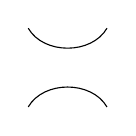
\begin{tikzpicture}[baseline={([yshift=-3pt]current bounding box.center)}]
    \draw (0,0) to [bend left=60] (1,0);
    \draw (0,1) to [bend right=60] (1,1);
\end{tikzpicture}%
}

% H pattern (horizontal connection)
\newcommand{\TLhorizontal}{%
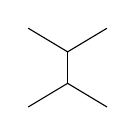
\begin{tikzpicture}[baseline={([yshift=-3pt]current bounding box.center)}]
    \draw (0,0) to (0.5,0.3) to (1,0);
    \draw (0,1) to (0.5,0.7) to (1,1);
    \draw (0.5,0.3) to (0.5,0.7);
\end{tikzpicture}%
}

% ============================================================
% Environment for Full Pentagon Diagram
% ============================================================
% Use the standalone file tex/figures/src/pentagon.tex for the full diagram
% or include inline with the patterns established above.

% ============================================================
% Environment for Full Hexagon Diagram
% ============================================================
% Use the standalone file tex/figures/src/hexagon.tex for the full diagram
% The hexagon.tex in literature/tex provides comprehensive examples.


% %%%%%%%%%%%%%%%%%%%%%%%%%%%%%%%%%%%%%%%%%%%%%%%%%%%%%%%%%%%%
% TRIVALENT CATEGORY DIAGRAMS
% %%%%%%%%%%%%%%%%%%%%%%%%%%%%%%%%%%%%%%%%%%%%%%%%%%%%%%%%%%%%
% For categories generated by a rotationally invariant trivalent vertex.
% These diagrams are unoriented and unlabeled (all strands carry object X).
% Key parameters: d (loop), b (bigon), t (triangle)

% ============================================================
% Trivalent Basic Relations
% ============================================================

% ------------------------------------------------------------
% Trivalent Loop: closed loop = d (quantum dimension)
% Usage: \trivloop (inline), or use in equations
% ------------------------------------------------------------
\newcommand{\trivloop}{%
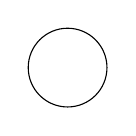
\begin{tikzpicture}[baseline=(current bounding box.center)]
    \draw (0,0) circle[radius=0.5cm];
\end{tikzpicture}%
}

% Loop with equals sign for relations
\newcommand{\trivloopeq}{%
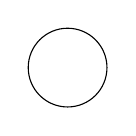
\begin{tikzpicture}[baseline=(current bounding box.center)]
    \draw (0,0) circle[radius=0.5cm];
\end{tikzpicture}\ = d%
}

% ------------------------------------------------------------
% Lollipop (forbidden diagram in trivalent categories)
% Usage: \trivlollipop = 0
% ------------------------------------------------------------
\newcommand{\trivlollipop}{%
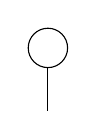
\begin{tikzpicture}[baseline=(current bounding box.center)]
    \draw (0,0) circle[radius=0.25cm];
    \draw (0,-0.25) -- (0,-0.8);
\end{tikzpicture}%
}

% ------------------------------------------------------------
% Trivalent Bigon: bigon = b * identity
% Usage: \trivbigon, \trivbigoneq
% ------------------------------------------------------------
\newcommand{\trivbigon}{%
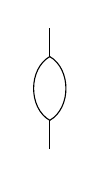
\begin{tikzpicture}[scale=0.9,baseline=(current bounding box.center)]
    \draw (0,-0.1) -- (0,0.3);
    \draw (0,0.3) to [bend left=60] (0,1.2);
    \draw (0,0.3) to [bend right=60] (0,1.2);
    \draw (0,1.2) -- (0,1.6);
\end{tikzpicture}%
}

\newcommand{\trivbigoneq}{%
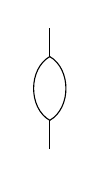
\begin{tikzpicture}[scale=0.9,baseline=(current bounding box.center)]
    \draw (0,-0.1) -- (0,0.3);
    \draw (0,0.3) to [bend left=60] (0,1.2);
    \draw (0,0.3) to [bend right=60] (0,1.2);
    \draw (0,1.2) -- (0,1.6);
\end{tikzpicture}\ = b \cdot\
\begin{tikzpicture}[scale=0.9,baseline=(current bounding box.center)]
    \draw (0,-0.1) -- (0,1.6);
\end{tikzpicture}%
}

% ------------------------------------------------------------
% Trivalent Triangle: triangle with external legs = t * trivalent vertex
% Usage: \trivtriangle, \trivtriangleeq
% ------------------------------------------------------------
\newcommand{\trivtriangle}{%
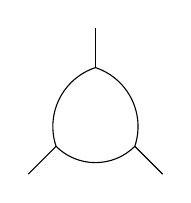
\begin{tikzpicture}[baseline=(current bounding box.center)]
    \draw (0.5,1) -- (0.5,1.5);
    \draw (0.5,1) to [bend right=45] (0,0);
    \draw (0.5,1) to [bend left=45] (1,0);
    \draw (0,0) to [bend right=45] (1,0);
    \draw (0,0) -- ++(225:0.5cm);
    \draw (1,0) -- ++(315:0.5cm);
\end{tikzpicture}%
}

\newcommand{\trivtriangleeq}{%
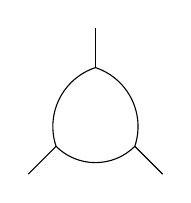
\begin{tikzpicture}[baseline=(current bounding box.center)]
    \draw (0.5,1) -- (0.5,1.5);
    \draw (0.5,1) to [bend right=45] (0,0);
    \draw (0.5,1) to [bend left=45] (1,0);
    \draw (0,0) to [bend right=45] (1,0);
    \draw (0,0) -- ++(225:0.5cm);
    \draw (1,0) -- ++(315:0.5cm);
\end{tikzpicture}\ = t \cdot\
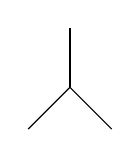
\begin{tikzpicture}[baseline=(current bounding box.center)]
    \draw (0,0) -- (90:0.75cm);
    \draw (0,0) -- (225:0.75cm);
    \draw (0,0) -- (315:0.75cm);
\end{tikzpicture}%
}

% ------------------------------------------------------------
% Trivalent Square: square face with external legs
% Usage: \trivsquare
% ------------------------------------------------------------
\newcommand{\trivsquare}{%
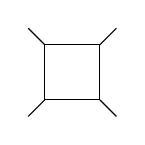
\begin{tikzpicture}[scale=0.7,baseline=(current bounding box.center)]
    \draw (0,0) rectangle (1,1);
    \draw (0,0) -- (-0.3,-0.3);
    \draw (0,1) -- (-0.3,1.3);
    \draw (1,0) -- (1.3,-0.3);
    \draw (1,1) -- (1.3,1.3);
\end{tikzpicture}%
}

% ============================================================
% C_4 Basis Diagrams (4 boundary points, no internal faces)
% These form a basis for Hom(1, X^4) in cubic trivalent categories
% ============================================================

% w_1: Two parallel vertical bigons (||)
\newcommand{\Cfourone}{%
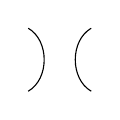
\begin{tikzpicture}[scale=0.5,baseline=(current bounding box.center)]
    \draw (-0.3,-0.3) to [bend right=60] (-0.3,1.3);
    \draw (1.3,-0.3) to [bend left=60] (1.3,1.3);
\end{tikzpicture}%
}

% w_2: Two horizontal bigons (=)
\newcommand{\Cfourtwo}{%
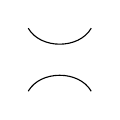
\begin{tikzpicture}[scale=0.5,baseline=(current bounding box.center)]
    \draw (-0.3,-0.3) to [bend left=60] (1.3,-0.3);
    \draw (-0.3,1.3) to [bend right=60] (1.3,1.3);
\end{tikzpicture}%
}

% w_3: H-pattern (horizontal connection)
\newcommand{\Cfourthree}{%
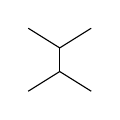
\begin{tikzpicture}[scale=0.5,baseline=(current bounding box.center)]
    \draw (-0.3,-0.3) to (0.5,0.2) to (1.3,-0.3);
    \draw (-0.3,1.3) to (0.5,0.8) to (1.3,1.3);
    \draw (0.5,0.2) to (0.5,0.8);
\end{tikzpicture}%
}

% w_4: I-pattern (vertical connection)
\newcommand{\Cfourfour}{%
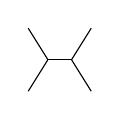
\begin{tikzpicture}[scale=0.5,baseline=(current bounding box.center)]
    \draw (-0.3,-0.3) to (0.2,0.5) to (-0.3,1.3);
    \draw (1.3,-0.3) to (0.8,0.5) to (1.3,1.3);
    \draw (0.2,0.5) to (0.8,0.5);
\end{tikzpicture}%
}

% ------------------------------------------------------------
% Square decomposition equation
% Usage: \trivsquaredecomp (shows alpha/beta coefficients)
% ------------------------------------------------------------
\newcommand{\trivsquaredecomp}{%
\trivsquare\ =\ \alpha\left(\Cfourone + \Cfourtwo\right) + \beta\left(\Cfourthree + \Cfourfour\right)%
}

% ============================================================
% Inner Product Pairing for Trivalent Diagrams
% Connects n boundary points of two diagrams
% ============================================================

% Generic inner product template (n=4 shown)
\newcommand{\trivinnerprod}[2]{%
\begin{tikzpicture}[baseline=(current bounding box.center)]
    \draw (2.1,0) arc(0:180:1.1);
    \draw (2.3,0) arc(0:180:1.3);
    \draw (1.7,0) arc(0:180:0.7);
    \node[rotate=90] at (1,0.9) {$\cdots$};
    \node [circle,draw,minimum size=1cm,text centered,fill=LightGray] at (0,0) {$#1$};
    \node [circle,draw,minimum size=1cm,text centered,fill=LightGray] at (2,0) {$#2$};
\end{tikzpicture}%
}

% ============================================================
% C_5 Basis Diagrams (5 boundary points)
% Representative patterns with 5-fold symmetry
% ============================================================

% 5-point diagram: two arcs with central trivalent vertex
\newcommand{\Cfivestar}{%
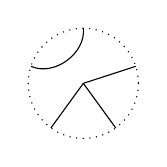
\begin{tikzpicture}[scale=0.7,baseline=(current bounding box.center)]
    \draw[dotted] (0,0) circle(1cm);
    \draw (90:1cm) to [bend left=60] (162:1cm);
    \draw (234:1cm) -- (0,0);
    \draw (306:1cm) -- (0,0);
    \draw (18:1cm) -- (0,0);
\end{tikzpicture}%
}

% 5-point diagram: chain pattern
\newcommand{\Cfivechain}{%
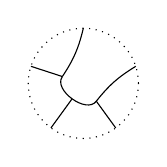
\begin{tikzpicture}[scale=0.7,baseline=(current bounding box.center)]
    \draw[dotted] (0,0) circle(1cm);
    \draw (90:1cm) to [bend left=10] (162:0.4cm);
    \draw (18:1cm) to [bend right=10] (306:0.4cm);
    \draw (162:0.4cm) to [bend right=90] (306:0.4cm);
    \draw (306:0.4cm) -- (306:1cm);
    \draw (162:0.4cm) -- (162:1cm);
    \draw (234:0.35cm) -- (234:1cm);
\end{tikzpicture}%
}

% Pentagon face with 5 external legs
\newcommand{\Cfivepentagon}{%
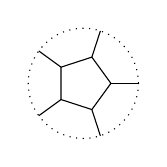
\begin{tikzpicture}[scale=0.7,baseline=(current bounding box.center)]
    \draw[dotted] (0,0) circle(1cm);
    \draw (0:0.5cm) -- (72:0.5cm) -- (144:0.5cm) -- (216:0.5cm) -- (288:0.5cm) -- cycle;
    \draw (0:0.5cm) -- (0:1cm);
    \draw (72:0.5cm) -- (72:1cm);
    \draw (144:0.5cm) -- (144:1cm);
    \draw (216:0.5cm) -- (216:1cm);
    \draw (288:0.5cm) -- (288:1cm);
\end{tikzpicture}%
}

% ============================================================
% C_6 Basis Diagrams (6 boundary points)
% Representative patterns for hexagonal symmetry
% ============================================================

% 6-point: three parallel bigons
\newcommand{\Csixthreebigon}{%
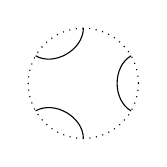
\begin{tikzpicture}[scale=0.7,baseline=(current bounding box.center)]
    \draw[dotted] (0,0) circle(1cm);
    \draw (90:1cm) to [bend left=60] (150:1cm);
    \draw (210:1cm) to [bend left=60] (270:1cm);
    \draw (330:1cm) to [bend left=60] (30:1cm);
\end{tikzpicture}%
}

% 6-point: two trivalent vertices connected
\newcommand{\Csixdumbbell}{%
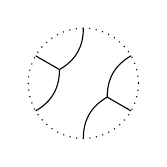
\begin{tikzpicture}[scale=0.7,baseline=(current bounding box.center)]
    \draw[dotted] (0,0) circle(1cm);
    \draw (150:1cm) -- (150:0.5cm);
    \draw (90:1cm) to [bend left=30] (150:0.5cm);
    \draw (210:1cm) to [bend right=30] (150:0.5cm);
    \draw (330:1cm) -- (330:0.5cm);
    \draw (270:1cm) to [bend left=30] (330:0.5cm);
    \draw (30:1cm) to [bend right=30] (330:0.5cm);
\end{tikzpicture}%
}

% Hexagon face with 6 external legs
\newcommand{\Csixhexagon}{%
\begin{tikzpicture}[scale=0.7,baseline=(current bounding box.center)]
    \draw[dotted] (0,0) circle(1cm);
    \draw (90:0.5cm) -- (150:0.5cm) -- (210:0.5cm) -- (270:0.5cm) -- (330:0.5cm) -- (30:0.5cm) -- cycle;
    \foreach \a in {30,90,...,330}
        \draw (\a:0.5cm) -- (\a:1cm);
\end{tikzpicture}%
}

% Pentafork: pentagon with one bigon attached
\newcommand{\Csixpentafork}{%
\begin{tikzpicture}[scale=0.7,baseline=(current bounding box.center)]
    \draw[dotted] (0,0) circle(1cm);
    \draw (210:1cm) to [bend left=60] (270:1cm);
    \draw (240:0.15cm) -- (240:0.5cm);
    \begin{scope}[scale=0.65,shift={(60:0.3)}]
        \draw (240:0.5) -- (312:0.5) -- (24:0.5) -- (96:0.5) -- (168:0.5) -- cycle;
    \end{scope}
    \draw (330:1cm) to ([scale=0.65,shift={(60:0.3)}]312:0.5);
    \draw (30:1cm) to ([scale=0.65,shift={(60:0.3)}]24:0.5);
    \draw (90:1cm) to ([scale=0.65,shift={(60:0.3)}]96:0.5);
    \draw (150:1cm) to ([scale=0.65,shift={(60:0.3)}]168:0.5);
\end{tikzpicture}%
}

% ============================================================
% 2-Local Hamiltonian Diagrams
% For nearest-neighbor interactions in anyon chains
% ============================================================

% Two-site identity (parallel strands)
% Baseline set for proper vertical centering in \left( \right) brackets
\newcommand{\Htwoidentity}{%
\begin{tikzpicture}[scale=0.6,baseline={([yshift=-0.5ex]current bounding box.center)}]
    \draw (0,0) -- (0,1.5);
    \draw (1,0) -- (1,1.5);
\end{tikzpicture}%
}

% Two-site swap (crossing strands)
\newcommand{\Htwoswap}{%
\begin{tikzpicture}[scale=0.6,baseline={([yshift=-0.5ex]current bounding box.center)}]
    \draw (0,0) -- (1,1.5);
    \draw (1,0) -- (0,1.5);
\end{tikzpicture}%
}

% Two-site cup-cap (TL generator)
\newcommand{\Htwocupcap}{%
\begin{tikzpicture}[scale=0.6,baseline={([yshift=-0.5ex]current bounding box.center)}]
    \draw (0,0) to [bend left=60] (1,0);
    \draw (0,1.5) to [bend right=60] (1,1.5);
\end{tikzpicture}%
}

% Two-site H-pattern (fusion-splitting)
\newcommand{\HtwoH}{%
\begin{tikzpicture}[scale=0.6,baseline={([yshift=-0.5ex]current bounding box.center)}]
    \draw (0,0) -- (0.5,0.4);
    \draw (1,0) -- (0.5,0.4);
    \draw (0.5,0.4) -- (0.5,1.1);
    \draw (0,1.5) -- (0.5,1.1);
    \draw (1,1.5) -- (0.5,1.1);
\end{tikzpicture}%
}

% Two-site with intermediate label
% Properly centered in brackets for Hamiltonian expressions
\newcommand{\Htwofusion}[1]{%
\begin{tikzpicture}[scale=0.6,baseline={([yshift=-0.5ex]current bounding box.center)}]
    \draw (0,0) -- (0.5,0.4);
    \draw (1,0) -- (0.5,0.4);
    \draw (0.5,0.4) -- (0.5,1.1) node[midway,right] {\tiny $#1$};
    \draw (0,1.5) -- (0.5,1.1);
    \draw (1,1.5) -- (0.5,1.1);
\end{tikzpicture}%
}

% Two-site braiding (over-crossing) - compact for Hamiltonians
\newcommand{\Htwobraid}{%
\begin{tikzpicture}[scale=0.6,baseline={([yshift=-0.5ex]current bounding box.center)}]
    \begin{knot}[flip crossing/.list={1},consider self intersections=true,ignore endpoint intersections=false,clip width=4]
        \strand (0,0) to[out=90,in=270] (1,1.5);
        \strand (1,0) to[out=90,in=270] (0,1.5);
    \end{knot}
\end{tikzpicture}%
}

% Two-site inverse braiding (under-crossing) - compact for Hamiltonians
\newcommand{\Htwobraidinv}{%
\begin{tikzpicture}[scale=0.6,baseline={([yshift=-0.5ex]current bounding box.center)}]
    \begin{knot}[consider self intersections=true,ignore endpoint intersections=false,clip width=4]
        \strand (0,0) to[out=90,in=270] (1,1.5);
        \strand (1,0) to[out=90,in=270] (0,1.5);
    \end{knot}
\end{tikzpicture}%
}

% Two-site hop RIGHT: anyon hops right (vacuum on left shown dashed)
% Left strand is vacuum (dashed), right strand is anyon (solid)
\newcommand{\Htwohopright}{%
\begin{tikzpicture}[scale=0.6,baseline={([yshift=-0.5ex]current bounding box.center)}]
    \begin{knot}[flip crossing/.list={1},consider self intersections=true,ignore endpoint intersections=false,clip width=4]
        \strand[dashed] (0,0) to[out=90,in=270] (1,1.5);
        \strand (1,0) to[out=90,in=270] (0,1.5);
    \end{knot}
\end{tikzpicture}%
}

% Two-site hop LEFT: anyon hops left (vacuum on right shown dashed)
% Left strand is anyon (solid), right strand is vacuum (dashed)
\newcommand{\Htwohopleft}{%
\begin{tikzpicture}[scale=0.6,baseline={([yshift=-0.5ex]current bounding box.center)}]
    \begin{knot}[flip crossing/.list={1},consider self intersections=true,ignore endpoint intersections=false,clip width=4]
        \strand (0,0) to[out=90,in=270] (1,1.5);
        \strand[dashed] (1,0) to[out=90,in=270] (0,1.5);
    \end{knot}
\end{tikzpicture}%
}

% Inverse hop RIGHT (under-crossing version)
\newcommand{\Htwohoprghtinv}{%
\begin{tikzpicture}[scale=0.6,baseline={([yshift=-0.5ex]current bounding box.center)}]
    \begin{knot}[consider self intersections=true,ignore endpoint intersections=false,clip width=4]
        \strand[dashed] (0,0) to[out=90,in=270] (1,1.5);
        \strand (1,0) to[out=90,in=270] (0,1.5);
    \end{knot}
\end{tikzpicture}%
}

% Inverse hop LEFT (under-crossing version)
\newcommand{\Htwohopleftinv}{%
\begin{tikzpicture}[scale=0.6,baseline={([yshift=-0.5ex]current bounding box.center)}]
    \begin{knot}[consider self intersections=true,ignore endpoint intersections=false,clip width=4]
        \strand (0,0) to[out=90,in=270] (1,1.5);
        \strand[dashed] (1,0) to[out=90,in=270] (0,1.5);
    \end{knot}
\end{tikzpicture}%
}

% ============================================================
% Chain Diagrams with Context
% Show local operators in the context of a chain
% ============================================================

% Local operator in chain context (dots ... O ... dots)
% Box drawn explicitly so strands connect exactly to edges
\newcommand{\chainlocal}[1]{%
\begin{tikzpicture}[scale=0.6,baseline=(current bounding box.center)]
    \node at (-0.5,0.75) {$\cdots$};
    % Left neighbor strand (passes through)
    \draw (0,0) -- (0,1.5);
    % Draw box explicitly with known coordinates
    \fill[LightGray] (0.35,0.4) rectangle (1.15,1.1);
    \draw (0.35,0.4) rectangle (1.15,1.1);
    \node at (0.75,0.75) {\tiny $#1$};
    % Two strands that connect TO the box (not through it)
    \draw (0.5,0) -- (0.5,0.4);      % bottom to box bottom
    \draw (0.5,1.1) -- (0.5,1.5);    % box top to top
    \draw (1.0,0) -- (1.0,0.4);      % bottom to box bottom
    \draw (1.0,1.1) -- (1.0,1.5);    % box top to top
    % Right neighbor strand (passes through)
    \draw (1.5,0) -- (1.5,1.5);
    \node at (2,0.75) {$\cdots$};
\end{tikzpicture}%
}

% ============================================================
% END OF TIKZ STYLE LIBRARY
% ============================================================
